\documentclass[11pt,a4paper,fontset=none]{ctexart}
\usepackage{fontspec}
\usepackage{xeCJK}
\usepackage{amsmath,amssymb,mathtools}
\usepackage{geometry}
\usepackage[dvipsnames]{xcolor}
\usepackage{tikz}
\usetikzlibrary{
  arrows.meta,
  angles,
  backgrounds,
  calc,
  decorations.markings,
  decorations.pathmorphing,
  decorations.pathreplacing,
  fit,
  intersections,
  matrix,
  patterns,
  patterns.meta,
  positioning,
  quotes,
  shapes.geometric,
  shapes.misc,
  through,
  3d
}
\usepackage{pgfplots}
\pgfplotsset{compat=1.18}
\usepackage[most]{tcolorbox}
\usepackage{enumitem}
\usepackage{multicol}
\usepackage{tabularx,array,booktabs,multirow}
\usepackage{fancyhdr}
\usepackage{lastpage}
\usepackage{titlesec}
\usepackage{needspace}
\usepackage{eso-pic}
\usepackage{graphicx}
\usepackage{hyperref}
\usepackage{xparse}

\geometry{
  a4paper,
  left=18mm,
  right=18mm,
  top=22mm,
  bottom=20mm,
  headheight=22pt,
  headsep=8mm,
  footskip=11mm
}

\setmainfont{texgyrepagella-regular.otf}[
  BoldFont=texgyrepagella-bold.otf,
  ItalicFont=texgyrepagella-italic.otf,
  BoldItalicFont=texgyrepagella-bolditalic.otf
]
\setsansfont{texgyreheros-regular.otf}[
  BoldFont=texgyreheros-bold.otf,
  ItalicFont=texgyreheros-italic.otf,
  BoldItalicFont=texgyreheros-bolditalic.otf
]
\setmonofont{texgyrecursor-regular.otf}[
  BoldFont=texgyrecursor-bold.otf
]
\setCJKmainfont{Kaiti SC}[
  BoldFont=Kaiti SC
]
\setCJKsansfont{FandolHei-Regular.otf}[
  BoldFont=FandolHei-Bold.otf
]
\setCJKmonofont{FandolKai-Regular.otf}

\definecolor{Paper}{HTML}{FBFCFA}
\definecolor{Ink}{HTML}{17324D}
\definecolor{Muted}{HTML}{647784}
\definecolor{Teal}{HTML}{167D89}
\definecolor{TealDark}{HTML}{0F5F69}
\definecolor{Mint}{HTML}{E8F5F2}
\definecolor{Sky}{HTML}{EAF3F8}
\definecolor{Coral}{HTML}{E66A5A}
\definecolor{Gold}{HTML}{D7A94A}
\definecolor{Rule}{HTML}{C8D8DA}
\definecolor{SolutionBg}{HTML}{FFF9F1}

\pagecolor{Paper}
\color{Ink}
\linespread{1.14}
\setlength{\parindent}{2em}
\setlength{\parskip}{0.25em}
\setlength{\columnsep}{1.3cm}
\setlength{\abovedisplayskip}{0.7em}
\setlength{\belowdisplayskip}{0.7em}
\setlist{nosep}

\hypersetup{
  colorlinks=true,
  linkcolor=TealDark,
  urlcolor=TealDark,
  pdfborder={0 0 0}
}

\newcommand{\papertitle}{Mathstalents 小学版练习题}
\newcommand{\SetPaperTitle}[1]{\renewcommand{\papertitle}{#1}}

\pagestyle{fancy}
\fancyhf{}
\fancyhead[L]{\sffamily\small\color{TealDark}\papertitle}
\fancyhead[R]{}
\fancyfoot[C]{%
  {\sffamily\scriptsize\color{Muted}第~\arabic{page}~页~/~共~\pageref*{LastPage}~页}%
}
\renewcommand{\headrulewidth}{0.4pt}
\renewcommand{\footrulewidth}{0pt}
\renewcommand{\headrule}{\hbox to\headwidth{\color{Rule}\leaders\hrule height \headrulewidth\hfill}}

\AddToShipoutPictureBG{%
  \begin{tikzpicture}[remember picture,overlay]
    \draw[Rule,line width=0.35pt,rounded corners=2pt]
      ([xshift=6mm,yshift=-6mm]current page.north west)
      rectangle
      ([xshift=-6mm,yshift=6mm]current page.south east);
    \draw[Teal,line width=1.1pt]
      ([xshift=6mm,yshift=-14mm]current page.north west) --
      ([xshift=6mm,yshift=-6mm]current page.north west) --
      ([xshift=14mm,yshift=-6mm]current page.north west);
    \draw[Coral,line width=1.1pt]
      ([xshift=-6mm,yshift=14mm]current page.south east) --
      ([xshift=-6mm,yshift=6mm]current page.south east) --
      ([xshift=-14mm,yshift=6mm]current page.south east);
  \end{tikzpicture}%
}

\newcommand{\metachip}[2][Teal]{%
  \tikz[baseline=(chip.base)]\node[
    fill=#1!10,
    draw=#1!45,
    text=#1!80!black,
    rounded corners=2.5pt,
    inner xsep=6pt,
    inner ysep=2.4pt,
    font=\sffamily\scriptsize
  ] (chip) {\textbf{#2}};%
}

\NewDocumentCommand{\makecover}{m m m m m m}{%
  \thispagestyle{empty}
  \begin{tikzpicture}[remember picture,overlay]
    \draw[Teal!14,line width=0.8pt,step=10mm]
      ([xshift=8mm,yshift=8mm]current page.south west) grid
      ([xshift=-8mm,yshift=-8mm]current page.north east);
    \node[
      anchor=north west,
      text=Ink,
      align=left,
      text width=155mm
    ] at ([xshift=24mm,yshift=-35mm]current page.north west) {
      {\sffamily\bfseries\fontsize{14}{18}\selectfont
        MATHSTALENTS \(\cdot\) ELEMENTARY}\\[9mm]
      {\sffamily\bfseries\fontsize{34}{42}\selectfont
        小学版 \(\,\boldsymbol{\cdot}\,\) #1}\\[3mm]
      {\sffamily\fontsize{17}{23}\selectfont
        练习题与参考答案}\\[11mm]
      {\color{TealDark}\rule{112mm}{1.1pt}}\\[7mm]
      {\sffamily\fontsize{13}{20}\selectfont #2}
    };
    \node[
      anchor=north west,
      fill=white,
      draw=TealDark,
      line width=0.6pt,
      text opacity=1,
      rounded corners=5pt,
      inner sep=9mm,
      text width=137mm
    ] at ([xshift=24mm,yshift=-126mm]current page.north west) {
      \begin{minipage}{137mm}
        \sffamily
        \begin{tabularx}{\linewidth}{>{\centering\arraybackslash}X
          >{\centering\arraybackslash}X
          >{\centering\arraybackslash}X}
          {\color{TealDark}\bfseries\Large #3} &
          {\color{TealDark}\bfseries\Large #4} &
          {\color{TealDark}\bfseries\Large 精编}\\[-1mm]
          {\color{Muted}\small 总分} &
          {\color{Muted}\small 题目数} &
          {\color{Muted}\small 题解版本}
        \end{tabularx}
        \vspace{6mm}
        {\color{Rule}\hrule}
        \vspace{5mm}
        {\color{Ink}\bfseries 题型结构}\par
        \vspace{2mm}
        {\color{Muted}\small #5}
      \end{minipage}
    };
  \end{tikzpicture}
  \null
  \clearpage
}

\newcommand{\paperinfo}[3]{%
  \begin{tcolorbox}[
    enhanced,
    colback=Sky,
    colframe=Teal!40,
    boxrule=0.6pt,
    arc=3pt,
    left=5mm,right=5mm,top=4mm,bottom=4mm
  ]
    \sffamily
    \begin{tabularx}{\linewidth}{@{}X X X@{}}
      \textbf{姓名：}\rule{28mm}{0.4pt} &
      \textbf{用时：}\rule{22mm}{0.4pt} &
      \textbf{得分：}\rule{22mm}{0.4pt}\\[3mm]
      \multicolumn{3}{@{}l@{}}{\small\color{Muted}
        #1 \qquad #2 \qquad #3}
    \end{tabularx}
  \end{tcolorbox}
  \vspace{2mm}
}

\newcommand{\mtQuestionNeedspace}{8.2cm}
\newcommand{\mtBannerNeedspace}{6.8cm}
\newcommand{\mtQuestionBreakLines}{8}

\newcommand{\sectionbanner}[2]{%
  \Needspace{\mtBannerNeedspace}
  \begin{tcolorbox}[
    enhanced,
    colback=white,
    colframe=TealDark,
    boxrule=0.65pt,
    arc=2.5pt,
    left=4mm,right=4mm,top=2.6mm,bottom=2.6mm,
    before skip=3.2mm,
    after skip=2.2mm
  ]
    {\sffamily\bfseries\large\color{TealDark}#1\quad
     \sffamily\small #2}
  \end{tcolorbox}
}

\NewDocumentEnvironment{question}{m m}{%
  \Needspace{\mtQuestionNeedspace}
  \begin{tcolorbox}[
    enhanced,
    breakable,
    lines before break=\mtQuestionBreakLines,
    colback=white,
    colframe=Rule,
    boxrule=0.55pt,
    arc=3pt,
    left=5mm,right=5mm,top=5mm,bottom=4mm,
    before skip=4mm,
    after skip=4mm,
    title={\sffamily\bfseries 第 #1 题（ #2 分 ）},
    coltitle=TealDark,
    colbacktitle=white,
    fonttitle=\sffamily\bfseries,
    attach boxed title to top left={xshift=4mm,yshift=-2.8mm},
    boxed title style={
      colback=white,
      colframe=TealDark,
      arc=2.5pt,
      boxrule=0.65pt,
      left=3mm,right=3mm,top=1.5mm,bottom=1.5mm
    }
  ]
  \hypertarget{question:#1}{}%
  \vspace{1mm}
}{%
  \end{tcolorbox}
}

\ExplSyntaxOn
\seq_new:N \g_mt_choices_seq
\dim_new:N \l_mt_choice_max_dim
\dim_new:N \l_mt_choice_sum_dim
\dim_new:N \l_mt_choice_tmp_dim
\dim_new:N \l_mt_choice_label_dim
\box_new:N \l_mt_choice_box

\NewDocumentCommand{\choice}{m}
{
  \seq_gput_right:Nn \g_mt_choices_seq {#1}
}

\cs_new_protected:Npn \mt_set_choice_label_dim:
{
  \hbox_set:Nn \l_mt_choice_box
  {
    \textcolor{TealDark}{\bfseries E.}
    \hspace{0.45em}
  }
  \dim_set:Nn \l_mt_choice_label_dim { \box_wd:N \l_mt_choice_box }
}

\cs_new_protected:Npn \mt_choice_label:n #1
{
  \textcolor{TealDark}{\bfseries \int_to_Alph:n {#1}.}
}

\cs_new_protected:Npn \mt_typeset_choice:nn #1#2
{
  \mt_choice_label:n {#1}\hspace{0.45em}#2
}

\cs_new_protected:Npn \mt_typeset_choice_par:nn #1#2
{
  \par\noindent
  \hangindent = \l_mt_choice_label_dim
  \hangafter = 1
  \makebox[\l_mt_choice_label_dim][l]{ \mt_choice_label:n {#1} }
  #2
  \par
}

\cs_new_protected:Npn \mt_measure_choices:
{
  \dim_zero:N \l_mt_choice_max_dim
  \dim_zero:N \l_mt_choice_sum_dim
  \int_step_inline:nn { \seq_count:N \g_mt_choices_seq }
  {
    \hbox_set:Nn \l_mt_choice_box
    {
      \mt_typeset_choice:nn {##1} { \seq_item:Nn \g_mt_choices_seq {##1} }
    }
    \dim_set:Nn \l_mt_choice_tmp_dim { \box_wd:N \l_mt_choice_box }
    \dim_set:Nn \l_mt_choice_sum_dim { \l_mt_choice_sum_dim + \l_mt_choice_tmp_dim + 1.6em }
    \dim_set:Nn \l_mt_choice_max_dim
    {
      \dim_max:nn { \l_mt_choice_max_dim } { \l_mt_choice_tmp_dim }
    }
  }
}

\cs_new_protected:Npn \mt_print_choices:
{
  \mt_set_choice_label_dim:
  \mt_measure_choices:
  \par\nopagebreak\vspace{0.5em}
  \dim_compare:nNnTF { \l_mt_choice_sum_dim } < { \linewidth }
  {
    \noindent
    \int_step_inline:nn { \seq_count:N \g_mt_choices_seq }
    {
      \mbox
      {
        \mt_typeset_choice:nn {##1} { \seq_item:Nn \g_mt_choices_seq {##1} }
      }
      \hfill
    }
    \par
  }
  {
    \dim_compare:nNnTF { \l_mt_choice_max_dim + 0.6em } < { 0.5\linewidth }
    {
      \noindent
      \int_step_inline:nn { \seq_count:N \g_mt_choices_seq }
      {
        \begin{minipage}[t]{0.48\linewidth}
          \raggedright
          \mt_typeset_choice_par:nn {##1} { \seq_item:Nn \g_mt_choices_seq {##1} }
        \end{minipage}
        \int_if_odd:nTF {##1}
        { \hfill }
        { \par\vspace{0.38em} }
      }
      \int_if_odd:nT { \seq_count:N \g_mt_choices_seq } { \par }
    }
    {
      \int_step_inline:nn { \seq_count:N \g_mt_choices_seq }
      {
        \mt_typeset_choice_par:nn {##1} { \seq_item:Nn \g_mt_choices_seq {##1} }
        \vspace{0.28em}
      }
    }
  }
  \vspace{0.25em}
  \seq_gclear:N \g_mt_choices_seq
}

\NewDocumentEnvironment{choices}{}
{
  \seq_gclear:N \g_mt_choices_seq
}
{
  \mt_print_choices:
}

\NewDocumentEnvironment{multichoices}{}
{
  \seq_gclear:N \g_mt_choices_seq
}
{
  \mt_print_choices:
}
\ExplSyntaxOff

\NewDocumentCommand{\subquestion}{m m}{%
  \par\medskip
  \noindent
  \metachip[Coral]{#1 分}\hspace{0.7em}#2\par
}

\newcommand{\answerlineskip}{9mm}

\newcommand{\answerspace}{%
  \par\vspace{12mm}%
}

\newcommand{\answerline}{%
  \ifmmode
    \underline{\hspace{2.8cm}}%
  \else
    \ifvmode
      \par\vspace{\answerlineskip}%
      \noindent{\color{Ink}\rule{0.46\linewidth}{0.5pt}}%
      \par\vspace{2.5mm}%
    \else
      \underline{\hspace{2.8cm}}%
    \fi
  \fi
}

\NewDocumentCommand{\answerbox}{m}{%
  \par\vspace{3mm}
  \begin{tcolorbox}[
    enhanced,
    colback=white,
    colframe=Teal!38!Rule,
    boxrule=0.7pt,
    arc=2.5pt,
    left=3.5mm,
    right=3.5mm,
    top=3mm,
    bottom=3mm,
    height=#1,
    before skip=0pt,
    after skip=2mm
  ]
    \mbox{}
  \end{tcolorbox}
}

\NewDocumentEnvironment{solution}{m m m m}{%
  \Needspace{5.4cm}
  \begin{tcolorbox}[
    enhanced,
    breakable,
    lines before break=6,
    colback=white,
    colframe=Gold!65!Ink,
    boxrule=0.6pt,
    arc=3pt,
    left=5mm,right=5mm,top=5mm,bottom=4mm,
    before skip=4mm,
    after skip=4mm,
    title={\sffamily\bfseries 第 #1 题 \(\cdot\) 参考解答},
    coltitle=Ink,
    colbacktitle=white,
    fonttitle=\sffamily\bfseries,
    attach boxed title to top left={xshift=4mm,yshift=-2.8mm},
    boxed title style={
      colback=white,
      colframe=Gold!65!Ink,
      arc=2.5pt,
      boxrule=0.65pt,
      left=3mm,right=3mm,top=1.5mm,bottom=1.5mm
    }
  ]
  \hypertarget{solution:#1}{}%
  \vspace{1mm}
  \noindent
  \metachip[Coral]{答案：#2}\hspace{0.45em}
  \metachip[Gold]{难度：#3}\hspace{0.45em}
  \metachip[Teal]{#4}
  \par\medskip
}{%
  \end{tcolorbox}
}

\NewDocumentCommand{\analysis}{+m}{%
  \par\smallskip
  {\sffamily\bfseries\color{TealDark}思路分析}\par
  \vspace{1mm}
  #1
  \par\smallskip
}

\NewDocumentCommand{\methodsummary}{+m}{%
  \par\medskip
  \noindent
  {\sffamily\bfseries\color{TealDark}方法总结}\quad
  {\sffamily\color{Ink}#1}\par
}

\newcommand{\solutiondivider}{%
  \clearpage
}


\SetPaperTitle{自学稿 · 排列、组合与二项式定理}
\hypersetup{
  pdftitle={排列、组合与二项式定理},
  pdfauthor={自学稿}
}

\newcounter{worked}
\newcounter{drill}
\newcommand{\Worked}[1]{%
  \refstepcounter{worked}%
  \par\medskip
  \noindent{\sffamily\bfseries\color{TealDark}例~\theworked}\quad #1%
}
\newcommand{\Drill}[1]{%
  \refstepcounter{drill}%
  \par\medskip
  \noindent{\sffamily\bfseries\color{Coral}练~\thedrill}\quad #1%
}

\tikzset{
  pc/.style={circle,minimum size=17pt,inner sep=0pt,font=\small,text=Ink},
  hi/.style={pc,fill=Mint,draw=TealDark,line width=0.6pt,text=TealDark}
}

\begin{document}

\section*{排列、组合与二项式定理}

这份稿解决一类问题：互不相同的对象，按规则挑选或排队，一共有多少种。读的时候按节往下走。每一节先给能直接用的公式，再说明它为什么对，然后用一道例题把它用出来。

读完之后，应当能做这四件事。

\begin{enumerate}[leftmargin=1.6em,itemsep=0.28em]
  \item 判断题目计不计顺序，从而决定用排列还是用组合。
  \item 用手算 \(A_n^k\) 和 \(C_n^k\)，并说出二者相差的那个倍数是什么。
  \item 用「含不含某一个」写出组合数的递推，并在杨辉三角里找到它。
  \item 写出 \((a+b)^n\) 的通项，并求出指定某一项的系数。
\end{enumerate}

记号与现行高中课本相同：\(n!\) 是 \(1\times 2\times\cdots\times n\)，\(A_n^k\) 是从 \(n\) 个不同元素里取 \(k\) 个的排列数，\(C_n^k\) 是相应的组合数。字母 A 取自 arrangement。课本里取出的个数常写成上标 \(m\)，即 \(A_n^m\)，与这里的 \(k\) 是同一个位置。

\section*{一、先写清「一种」}

计数之前先写一句：怎样算一种结果。这句话定下来，后面的公式才有地方用。

一件事分成几类，类与类不重叠，合起来又盖住全部，总数是各类方法数之和。一件事要按顺序做完几步，每一步的做法都定下来才算完成，总数是各步方法数之积。

\begin{tcolorbox}[
  colback=Mint,colframe=TealDark,boxrule=0.6pt,arc=2pt,
  left=8pt,right=8pt,top=6pt,bottom=6pt
]
分类用加法，分步用乘法。交换两个选出的对象之后，若算另一种结果，就是排列；若仍算同一种，就是组合。
\end{tcolorbox}

\Worked{用 \(1,2,3\) 排成两位数，数字不重复。有多少个？}

百位有 \(3\) 种选法。百位定了之后，十位还有 \(2\) 种。两步都做完才得到一个两位数，所以是
\[
  3\times 2=6.
\]
六个数是 \(12,13,21,23,31,32\)。这里 \(12\) 和 \(21\) 是两个数，顺序被算进去了。

若改成「从 \(1,2,3\) 里取出两个数，不计谁先谁后」，则 \(\{1,2\}\) 只算一次。上面的六个两位数正好两两合成三对，取法是 \(3\) 种。同一批对象，问法不同，数就不同。

\section*{二、阶乘}

\(n\) 个不同对象排成一行，第一个位置有 \(n\) 种选法，第二个还有 \(n-1\) 种，最后一个只剩 \(1\) 种。分步相乘：
\[
  n!=n\times(n-1)\times\cdots\times 1.
\]
约定 \(0!=1\)。一个元素都没有时，排法只有「什么都不排」这一种。有了这个约定，\(k=n\) 时分母 \((n-n)!\) 有定义，组合公式在 \(k=0\) 时分母里的 \(k!\) 也有定义。前几个值是
\[
  0!=1,\quad 1!=1,\quad 2!=2,\quad 3!=6,\quad 4!=24,\quad 5!=120,\quad 6!=720.
\]

\section*{三、排列}

从 \(n\) 个不同元素里取出 \(k\) 个，排成一列。第一个位置有 \(n\) 种选法，第二个有 \(n-1\) 种，直到第 \(k\) 个位置有 \(n-k+1\) 种。因此
\[
  A_n^k=n(n-1)\cdots(n-k+1)=\frac{n!}{(n-k)!}.
\]
\(k=n\) 时，就是把全部元素排成一行，\(A_n^n=n!\)。\(k=0\) 时，\(A_n^0=1\)。

手算时直接连乘，不必先把两个阶乘都算出来。例如
\[
  A_8^3=8\times 7\times 6=336.
\]

\Worked{用 \(1,2,3,4,5\) 组成没有重复数字的三位数，有多少个？其中偶数有多少个？}

三位数计顺序，数字不重复，所以是排列：
\[
  A_5^3=5\times 4\times 3=60.
\]

偶数要看个位。个位可以是 \(2\) 或 \(4\)，两类相加。个位先定为 \(2\)，剩下两个位置从另外 \(4\) 个数字里排，有 \(A_4^2=12\) 个；个位定为 \(4\) 时同样有 \(12\) 个。偶数一共 \(24\) 个。

\Worked{用 \(0,1,2,3,4\) 组成没有重复数字的三位数，有多少个？}

\(0\) 不能放在百位。百位先从 \(1,2,3,4\) 里选，有 \(4\) 种；十位可以从剩下的 \(4\) 个数字里选（这时 \(0\) 已经允许）；个位再从剩下的 \(3\) 个里选。
\[
  4\times 4\times 3=48.
\]
同一件事也可以倒过来减：若允许 \(0\) 打头，有 \(A_5^3=60\) 个字符串；其中百位是 \(0\) 的有 \(A_4^2=12\) 个。真正的三位数是 \(60-12=48\)。两种算法应当一致。

\begin{tcolorbox}[
  colback=Sky,colframe=TealDark,boxrule=0.6pt,arc=2pt,
  left=8pt,right=8pt,top=6pt,bottom=6pt
]
\textbf{相邻与不相邻.}\quad
若干元素要求站在一起时，先把它们捆成一个整体，整体内部再排，然后与其余元素一起做全排列。要求某两个不相邻时，用全部排列减去这两个相邻的排法。

五本不同的书排成一排，语文和数学相邻：把这两本捆成一个整体，内部 \(2\) 种顺序，再与另外三本一共四个单位，排法是 \(2\times 4!=48\)。

二者不相邻：全部 \(5!=120\) 种，减去相邻的 \(48\) 种，得到 \(72\) 种。
\end{tcolorbox}

\section*{四、组合}

从 \(n\) 个不同元素里取出 \(k\) 个，只问取出哪几个，不问顺序。每一种取法对应 \(k!\) 种排法，因为取出之后还可以再排成一列。所以
\[
  C_n^k=\frac{A_n^k}{k!}=\frac{n!}{k!\,(n-k)!}.
\]
手算时写成连除，约分之后再乘：
\[
  C_n^k=\frac{n}{1}\cdot\frac{n-1}{2}\cdot\frac{n-2}{3}\cdots\frac{n-k+1}{k}.
\]
例如
\[
  C_8^3=\frac{8}{1}\cdot\frac{7}{2}\cdot\frac{6}{3}=56,\qquad
  C_{10}^{3}=\frac{10}{1}\cdot\frac{9}{2}\cdot\frac{8}{3}=120.
\]
\(C_n^0=1\)，\(C_n^n=1\)：什么都不取，只有一种；全部取走，也只有一种。

\begin{center}
\renewcommand{\arraystretch}{1.25}
\begin{tabular}{ccc}
组合 & 对应的排列 & 条数\\
\(\{\text{甲},\text{乙}\}\) & 甲乙，乙甲 & \(2!\)\\
\(\{\text{甲},\text{丙}\}\) & 甲丙，丙甲 & \(2!\)\\
\(\{\text{乙},\text{丙}\}\) & 乙丙，丙乙 & \(2!\)
\end{tabular}

\vspace{0.35em}
{\small 从甲、乙、丙里取 \(2\) 个：\(C_3^2=3\)，\(A_3^2=6\)，每个组合对应 \(2!\) 种排列。}
\end{center}

\Worked{八年级有 \(12\) 名同学，选出 \(3\) 人去办板报，有多少种选法？若甲必须入选，有多少种？}

办板报只看哪三个人，不计谁站左边，用组合：
\[
  C_{12}^{3}=\frac{12}{1}\cdot\frac{11}{2}\cdot\frac{10}{3}=220.
\]
甲已经入选，再从其余 \(11\) 人里选 \(2\) 人：
\[
  C_{11}^{2}=\frac{11\times 10}{2}=55.
\]

\Worked{从 \(1,2,\ldots,9\) 里任取两个数，和能被 \(3\) 整除的取法有多少种？}

两个数不计顺序，先用组合分类，分类标准是除以 \(3\) 的余数。余数是 \(0\) 的有 \(3,6,9\)；余数是 \(1\) 的有 \(1,4,7\)；余数是 \(2\) 的有 \(2,5,8\)。每组 \(3\) 个数。

两数之和能被 \(3\) 整除，就是两个余数之和能被 \(3\) 整除。两个余数相加，只有两种搭配成立：都是 \(0\)，因为 \(0+0=0\)；或者一个 \(1\)、一个 \(2\)，因为 \(1+2=3\)。

两个余数都是 \(1\) 时，\(1+1=2\)，和除以 \(3\) 余 \(2\)。两个余数都是 \(2\) 时，\(2+2=4\)，和除以 \(3\) 余 \(1\)。这两种的和都不能被 \(3\) 整除。

都是 \(0\)，是在余数 \(0\) 那一组里取两个：
\[
  C_3^2=3.
\]
一个 \(1\)、一个 \(2\)，是两组之间各取一个：\(3\times 3=9\)。合起来 \(12\) 种。全部取法是 \(C_9^2=36\)，\(12\) 正好是其中的三分之一。

\section*{五、组合数的两条性质}

\textbf{取走与留下是同一件事。}
从 \(n\) 个里取出 \(k\) 个，等于决定哪 \(n-k\) 个留下。两种说法一一对应，所以
\[
  C_n^k=C_n^{n-k}.
\]
计算时取较小的那个下标。\(C_{10}^{8}=C_{10}^{2}=45\)，比连乘八次省事。

\textbf{含不含某一个固定元素。}
把元素甲单独拿出来看。取 \(k\) 个的方法分成两类：甲在其中，则再从其余 \(n-1\) 个里取 \(k-1\) 个；甲不在其中，则从其余 \(n-1\) 个里取 \(k\) 个。两类不重叠，合起来是全部取法，所以
\[
  C_n^k=C_{n-1}^{k-1}+C_{n-1}^{k}.
\]
下标出界时，那个组合数记为 \(0\)。例如 \(k=0\) 时，第一项 \(C_{n-1}^{-1}=0\)，第二项 \(C_{n-1}^{0}=1\)，和仍是 \(1\)。

\Worked{用这条递推核对 \(C_5^2\)。}

\[
  C_5^2=C_4^1+C_4^2.
\]
\(C_4^1=4\)。\(C_4^2=C_3^1+C_3^2\)，而 \(C_3^1=3\)，\(C_3^2=C_3^1=3\)，所以 \(C_4^2=3+3=6\)。于是 \(C_5^2=4+6=10\)。直接计算是 \(\dfrac{5\times 4}{2}=10\)，两边一致。

\section*{六、杨辉三角}

把 \(C_n^k\) 按 \(n\) 分行、按 \(k\) 从左到右排，每一行的两端都是 \(1\)，中间每个数等于它肩上两数之和。这就是上一节的递推。第 \(n\) 行（从 \(0\) 数起）从左到右是
\[
  C_n^0,\; C_n^1,\; \ldots,\; C_n^n.
\]

\begin{center}
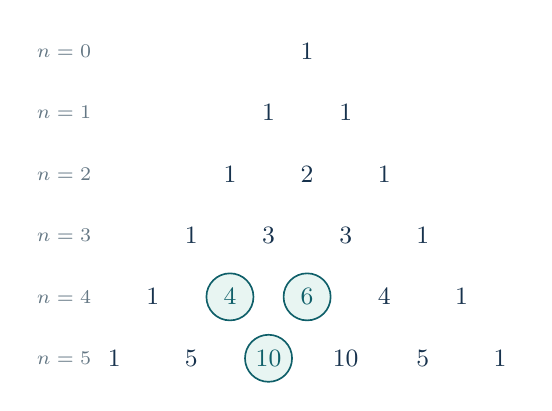
\begin{tikzpicture}[x=0.98cm,y=0.78cm]
  \node[font=\scriptsize,text=Muted] at (-3.15,0) {\(n=0\)};
  \node[font=\scriptsize,text=Muted] at (-3.15,-1) {\(n=1\)};
  \node[font=\scriptsize,text=Muted] at (-3.15,-2) {\(n=2\)};
  \node[font=\scriptsize,text=Muted] at (-3.15,-3) {\(n=3\)};
  \node[font=\scriptsize,text=Muted] at (-3.15,-4) {\(n=4\)};
  \node[font=\scriptsize,text=Muted] at (-3.15,-5) {\(n=5\)};
  \node[pc] at (0,0) {1};
  \node[pc] at (-0.5,-1) {1};
  \node[pc] at (0.5,-1) {1};
  \node[pc] at (-1,-2) {1};
  \node[pc] at (0,-2) {2};
  \node[pc] at (1,-2) {1};
  \node[pc] at (-1.5,-3) {1};
  \node[pc] at (-0.5,-3) {3};
  \node[pc] at (0.5,-3) {3};
  \node[pc] at (1.5,-3) {1};
  \node[pc] at (-2,-4) {1};
  \node[hi] at (-1,-4) {4};
  \node[hi] at (0,-4) {6};
  \node[pc] at (1,-4) {4};
  \node[pc] at (2,-4) {1};
  \node[pc] at (-2.5,-5) {1};
  \node[pc] at (-1.5,-5) {5};
  \node[hi] at (-0.5,-5) {10};
  \node[pc] at (0.5,-5) {10};
  \node[pc] at (1.5,-5) {5};
  \node[pc] at (2.5,-5) {1};
\end{tikzpicture}

\vspace{0.3em}
{\small 图\quad 杨辉三角的前六行。涂色的三个数是 \(C_4^1=4\)，\(C_4^2=6\)，以及它们的和 \(C_5^2=10\)。}
\end{center}

第 \(n\) 行全部加起来，是 \(n\) 元集合的子集个数。每个元素有「进这个子集」和「不进」两种选择，分步相乘得到 \(2^n\)。按子集的大小分类，大小为 \(k\) 的子集有 \(C_n^k\) 个，所以
\[
  \sum_{k=0}^{n}C_n^k=2^n.
\]
图中 \(n=4\) 的一行：\(1+4+6+4+1=16=2^4\)。

\section*{七、二项式定理}

\((a+b)^n\) 是 \(n\) 个 \((a+b)\) 相乘。展开之后，每一项都是从每个括号里取 \(a\) 或取 \(b\)，再乘起来。若有 \(k\) 个括号取了 \(b\)，其余 \(n-k\) 个括号取了 \(a\)，就得到 \(a^{n-k}b^k\)。哪 \(k\) 个括号取 \(b\)，有 \(C_n^k\) 种选法，这些选法给出的是同类项。因此
\[
  (a+b)^n=\sum_{k=0}^{n}C_n^k\,a^{n-k}b^k.
\]
\(k\) 从 \(0\) 数到 \(n\)。含 \(b^k\) 的那一项是展开式的第 \(k+1\) 项，
\[
  T_{k+1}=C_n^k\,a^{n-k}b^k.
\]
系数 \(C_n^k\) 正是杨辉三角第 \(n\) 行的第 \(k\) 个数（也从 \(0\) 数起）。所以 \((a+b)^4\) 的系数是 \(1,4,6,4,1\)：
\[
  (a+b)^4=a^4+4a^3b+6a^2b^2+4ab^3+b^4.
\]

\Worked{求 \((2x-1)^5\) 的展开式里 \(x^3\) 的系数。}

通项是
\[
  T_{k+1}=C_5^k\,(2x)^{5-k}(-1)^k
  =C_5^k\,2^{5-k}(-1)^k\,x^{5-k}.
\]
要让 \(x\) 的次数是 \(3\)，就让 \(5-k=3\)，得 \(k=2\)。这一项的系数是
\[
  C_5^2\cdot 2^{3}\cdot(-1)^{2}=10\times 8\times 1=80.
\]

\Worked{用代入说明偶数项之和与奇数项之和。}

令 \(a=1\)，\(b=1\)：
\[
  \sum_{k=0}^{n}C_n^k=(1+1)^n=2^n.
\]
这和第六节用子集数出来的是同一个数。再令 \(a=1\)，\(b=-1\)。当 \(n\ge 1\) 时，
\[
  \sum_{k=0}^{n}(-1)^k C_n^k=(1-1)^n=0.
\]
两式相加，\(k\) 为奇数的项互相抵消，\(k\) 为偶数的项各出现两次：
\[
  2\sum_{k\text{ 为偶数}}C_n^k=2^n.
\]
两式相减，\(k\) 为偶数的项抵消，留下
\[
  2\sum_{k\text{ 为奇数}}C_n^k=2^n.
\]
所以 \(n\ge 1\) 时，这两种和都是 \(2^{n-1}\)。这里的偶数、奇数指的是 \(k\)，不是从左数第几格。\(n=4\) 时，\(k\) 为偶数的是 \(C_4^0+C_4^2+C_4^4=1+6+1=8\)，\(k\) 为奇数的是 \(C_4^1+C_4^3=4+4=8\)。

\begin{tcolorbox}[
  colback=SolutionBg,colframe=Gold!80!black,boxrule=0.6pt,arc=2pt,
  left=8pt,right=8pt,top=6pt,bottom=6pt
]
\textbf{选用哪一个.}\quad
排成一列、组成数、分先后，用 \(A_n^k\)。只取一组、选一个委员会、配一对，用 \(C_n^k\)。先选出一组、再在组内分工，先用组合，再用排列或乘法。展开 \((a+b)^n\)、求某一项的系数，用二项式定理，系数就是 \(C_n^k\)。
\end{tcolorbox}

\section*{八、再走一步}

下面两条是主公式的紧邻用法。主线上的练习不依赖它们。

有重复对象时，全排列要除掉重复排法。\(n\) 个对象里，若有 \(a\) 个彼此相同，另有 \(b\) 个彼此相同，其余对象都互不相同，也和这两组不同，不同的排法是
\[
  \frac{n!}{a!\,b!}.
\]
单词 \(BOOK\) 有 \(4\) 个字母，其中两个 \(O\) 相同，\(B\) 和 \(K\) 各不相同，排法是 \(4!/2!=12\)。两个 \(O\) 互换之后看不出差别。

\(n\) 个不同的人围圆桌就座，旋转之后视为同一种坐法。把某一个人先固定为参照，其余 \(n-1\) 个人排列，种数是 \((n-1)!\)。

\section*{九、练习}

\Drill{计算 \(A_7^3\) 和 \(C_7^3\)。二者相除，商是多少？这个商在定义里代表什么？}

\Drill{用 \(0,1,2,3,4\) 组成没有重复数字的三位数。一共有多少个？其中能被 \(5\) 整除的有多少个？}

\Drill{从 \(8\) 名同学中选 \(3\) 名值日，有多少种选法？若甲必须参加，有多少种？}

\Drill{从 \(10\) 件各不相同的礼物中送出 \(4\) 件。说明送出 \(4\) 件与留下 \(6\) 件的种数为什么相同，并算出这个数。}

\Drill{写出 \((x+1)^5\) 的展开式。}

\Drill{求 \((x-2)^6\) 的展开式中 \(x^4\) 的系数。}

\Drill{五本不同的书排成一排，其中语文和数学不相邻，有多少种排法？}

\Drill{从 \(1,2,\ldots,9\) 中任取三个数，和能被 \(3\) 整除的取法有多少种？}

\section*{十、练习答案}

\textbf{练 1.}\quad
\(A_7^3=7\times 6\times 5=210\)，\(C_7^3=\dfrac{210}{6}=35\)。商是 \(3!=6\)，也就是把取出的 \(3\) 个元素再排成一列的排法数。

\textbf{练 2.}\quad
百位不能是 \(0\)，有 \(4\times 4\times 3=48\) 个。能被 \(5\) 整除时个位必须是 \(0\)（这五个数字里没有 \(5\)）。个位固定为 \(0\) 之后，百位、十位是 \(A_4^2=12\) 个。

\textbf{练 3.}\quad
\(C_8^3=\dfrac{8\times 7\times 6}{6}=56\)。甲必须参加时，再选 \(2\) 人，\(C_7^2=21\)。

\textbf{练 4.}\quad
送出的 \(4\) 件一旦定了，留下的 \(6\) 件也定了，两种数法是同一批结果，所以 \(C_{10}^{4}=C_{10}^{6}\)。
\[
  C_{10}^{4}=\frac{10\times 9\times 8\times 7}{4\times 3\times 2\times 1}=210.
\]

\textbf{练 5.}\quad
系数为 \(1,5,10,10,5,1\)，
\[
  (x+1)^5=x^5+5x^4+10x^3+10x^2+5x+1.
\]

\textbf{练 6.}\quad
通项 \(T_{k+1}=C_6^k\,x^{6-k}(-2)^k\)。令 \(6-k=4\)，得 \(k=2\)。系数是
\[
  C_6^2\cdot(-2)^2=15\times 4=60.
\]

\textbf{练 7.}\quad
全部排法 \(5!=120\)。语文和数学相邻时，捆绑后有 \(2\times 4!=48\) 种。不相邻的是 \(120-48=72\) 种。

\textbf{练 8.}\quad
按除以 \(3\) 的余数分组，每组 \(3\) 个数。三个余数之和是 \(3\) 的倍数，只有两类：三个余数相同，或者三个余数分别是 \(0,1,2\)。三个相同都可以：\(0+0+0=0\)，\(1+1+1=3\)，\(2+2+2=6\)。这和例 5 不同，两个数的余数都是 \(1\) 时和不能被 \(3\) 整除，三个数就可以。
\[
  C_3^3+C_3^3+C_3^3+3\times 3\times 3=1+1+1+27=30.
\]

\end{document}
